
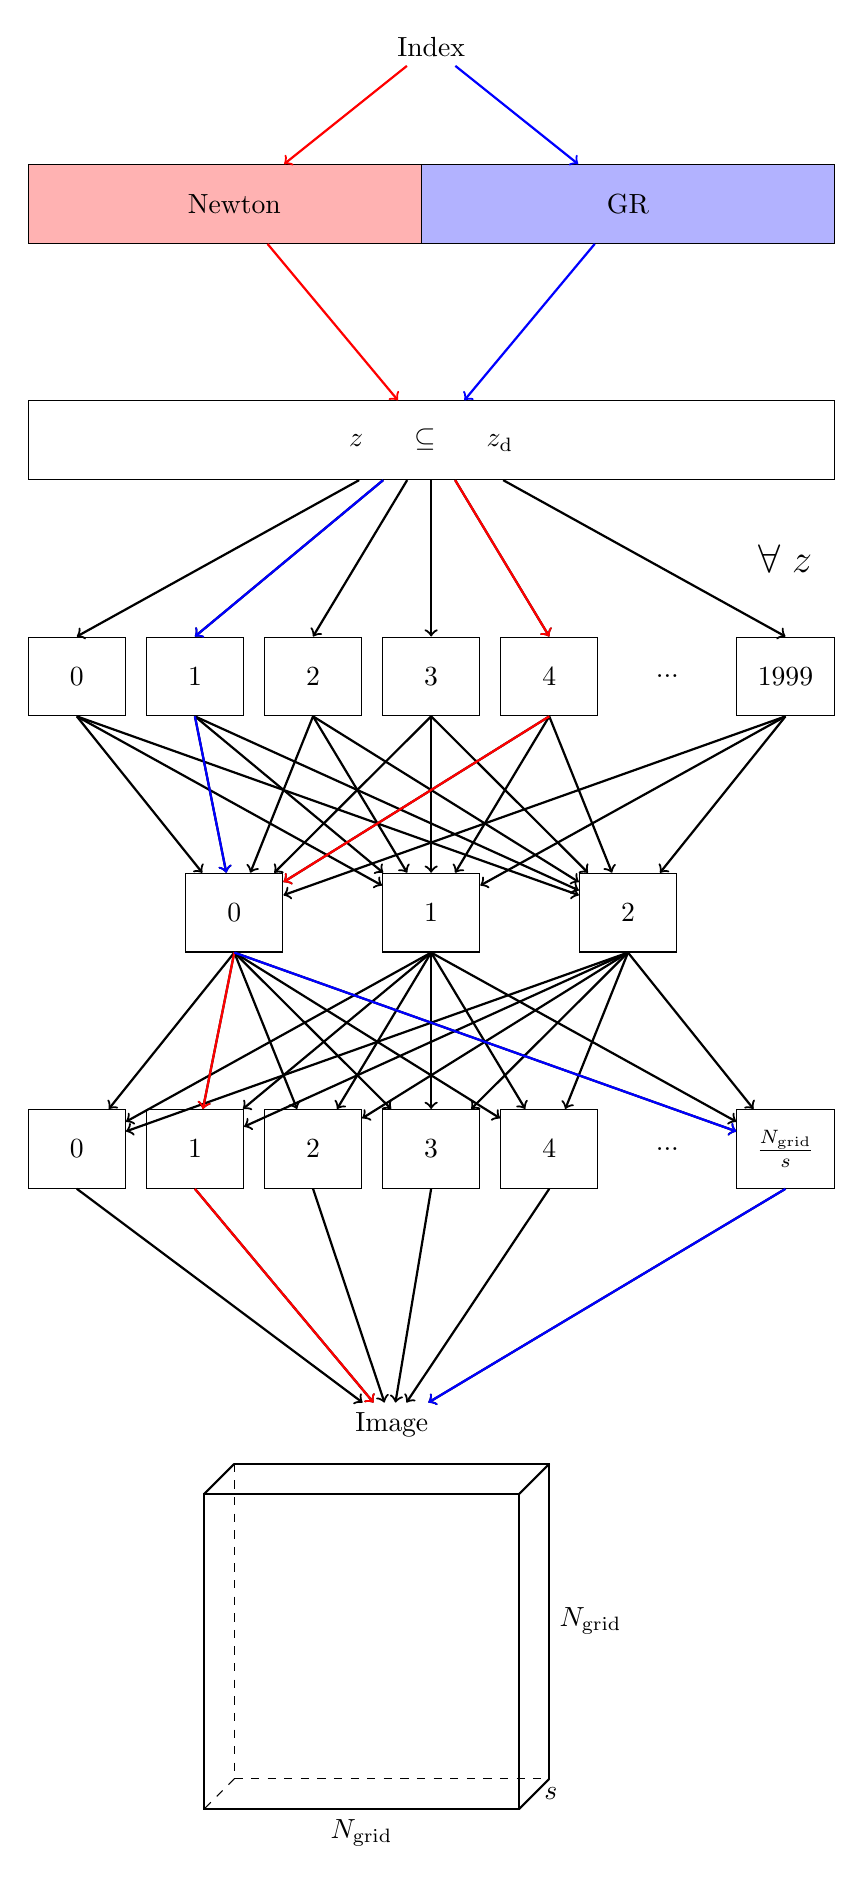
\begin{tikzpicture}
    % Index 
    \node (Index) at (2.5, 5) {Index};

    % Gravity theory
    \node[draw, rectangle, fill=red!30, text width=5cm, text centered, minimum height=1cm] (newton) at (0,3) {Newton};
    \node[draw, rectangle, fill=blue!30, text width=5cm, text centered, minimum height=1cm] (gr) at (5,3) {GR};

    % Redshifts
    \node[draw, rectangle, fill=white, text width=10cm, text centered, minimum height=1cm] (redshifts) at (2.5, 0) {$z\subseteq z_\mathrm{d}$};

    

    % Seeds
    \node[draw, rectangle, fill=white, text width=1cm, text centered, minimum height=1cm] (s1) at (-2,-3) {0};
    \node[draw, rectangle, fill=white, text width=1cm, text centered, minimum height=1cm] (s2) at (-0.5,-3) {1};
    \node[draw, rectangle, fill=white, text width=1cm, text centered, minimum height=1cm] (s3) at (1,-3) {2};
    \node[draw, rectangle, fill=white, text width=1cm, text centered, minimum height=1cm] (s4) at (2.5,-3) {3};
    \node[draw, rectangle, fill=white, text width=1cm, text centered, minimum height=1cm] (s5) at (4,-3) {4};
    \node at (5.5,-3) {...};
    \node[draw, rectangle, fill=white, text width=1cm, text centered, minimum height=1cm] (s1999) at (7,-3) {1999};

    \draw[->, thick] (redshifts) -- (s1.north);
    \draw[->, thick] (redshifts) -- (s2.north);
    \draw[->, thick] (redshifts) -- (s3.north);
    \draw[->, thick] (redshifts) -- (s4.north);
    \draw[->, thick] (redshifts) -- (s5.north);
    \draw[->, thick] (redshifts) -- (s1999.north);
    \node[font=\Large] at (7, -1.5) {$\forall \; z$};

    
    % Axes
    \node[draw, rectangle, fill=white, text width=1cm, text centered, minimum height=1cm] (ax1) at (0,-6) {0};
    \node[draw, rectangle, fill=white, text width=1cm, text centered, minimum height=1cm] (ax2) at (2.5,-6) {1};
    \node[draw, rectangle, fill=white, text width=1cm, text centered, minimum height=1cm] (ax3) at (5,-6) {2};

    \foreach \seed in {s1, s2, s3, s4, s5, s1999}{
        \foreach \ax in {ax1, ax2, ax3}{
            \draw[->, thick] (\seed.south) -- (\ax);
            }
    }
    
    % Slices
    \node[draw, rectangle, fill=white, text width=1cm, text centered, minimum height=1cm] (r1) at (-2,-9) {0};
    \node[draw, rectangle, fill=white, text width=1cm, text centered, minimum height=1cm] (r2) at (-0.5,-9) {1};
    \node[draw, rectangle, fill=white, text width=1cm, text centered, minimum height=1cm] (r3) at (1,-9) {2};
    \node[draw, rectangle, fill=white, text width=1cm, text centered, minimum height=1cm] (r4) at (2.5,-9) {3};
    \node[draw, rectangle, fill=white, text width=1cm, text centered, minimum height=1cm] (r5) at (4,-9) {4};
    \node at (5.5,-9) {...};
    \node[draw, rectangle, fill=white, text width=1cm, text centered, minimum height=1cm] (rend) at (7,-9) {$\frac{N_\mathrm{grid}}{s}$};
    
    \foreach \ax in {ax1, ax2, ax3}{
        \foreach \slices in {r1, r2, r3, r4, r5, rend}{
            \draw[->, thick] (\ax.south) -- (\slices);
        }
    }
            
            


    % Image
    \tdplotsetmaincoords{70}{110}
    \pgfmathsetmacro{\Nlength}{4}
    \pgfmathsetmacro{\stride}{1}
    \pgfmathsetmacro{\waybelow}{-17}

    % Draw 3d square
    \draw[dashed] (0,\waybelow,0) -- (\Nlength, \waybelow, 0);
    \draw[thick] (\Nlength, \waybelow, 0) -- (\Nlength, \waybelow+\Nlength, 0) node[midway, right] {$N_\mathrm{grid}$} -- (0, \waybelow+\Nlength, 0);
    \draw[dashed] (0, \waybelow+\Nlength, 0) -- (0, \waybelow, 0);
    \draw[thick] (0,\waybelow,\stride) -- (\Nlength, \waybelow,\stride) node[midway, below] {$N_\mathrm{grid}$} -- (\Nlength, \waybelow+\Nlength, \stride) -- (0, \waybelow+\Nlength, \stride) -- cycle;

    % Small lengths
    \draw[dashed] (0,\waybelow,0) -- (0,\waybelow, \stride);
    \draw[thick] (\Nlength,\waybelow,0) -- (\Nlength,\waybelow, \stride) node[midway, right] {$s$};
    \draw[thick] (\Nlength,\waybelow+\Nlength,0) -- (\Nlength,\waybelow+\Nlength, \stride);
    \draw[thick] (0,\waybelow+\Nlength,0) -- (0,\waybelow+\Nlength, \stride);

    \node (Image) at (2, -12.5) {Image};

    \foreach \slice in {r1, r2, r3, r4, r5, rend}{
        \draw[->, thick] (\slice.south) -- (Image);
    }

    % Newton path
    \draw[->, thick, red] (Index) -- (newton);
    \draw[->, thick, red] (newton) -- (redshifts);
    \draw[->, thick, red] (redshifts) -- (s5.north);
    \draw[->, thick, red] (s5.south) -- (ax1);
    \draw[->, thick, red] (ax1.south) -- (r2);
    \draw[->, thick, red] (r2.south) -- (Image);
    % GR path
    \draw[->, thick, blue] (Index) -- (gr);
    \draw[->, thick, blue] (gr) -- (redshifts);
    \draw[->, thick, blue] (redshifts) -- (s2.north);
    \draw[->, thick, blue] (s2.south) -- (ax1);
    \draw[->, thick, blue] (ax1.south) -- (rend);
    \draw[->, thick, blue] (rend.south) -- (Image);

\end{tikzpicture}
